%! Author = Marjan
%! Date = 16/06/2025
% Preamble
\documentclass[a4paper, 11pt]{book}

% Packages
\usepackage{amsmath}
\usepackage{geometry}
\usepackage{fancyhdr}
\usepackage{hyperref}
\usepackage[framemethod=tikz]{mdframed}
\usepackage{tikz}
\usepackage[utf8]{inputenc}
%\usepackage{beamerbasenotes}
%\usepackage[toc]{glossaries} % 'toc' adds the glossary to the table of contents
%\makeglossaries
\usetikzlibrary{positioning, arrows.meta, shapes.multipart}
\renewcommand{\rmdefault}{phv} % Set the default font family to Helvetica
% ---- Set page margins (A4 paper)
\geometry{top=1in, bottom=1in, left=1in, right=1in}

% ---- Set up the header
\pagestyle{fancy}
\fancyhf{}
\fancyhead[L]{Data Architecture Notes}
%\fancyhead[C]{Your Name}
\fancyhead[R]{\thepage}

% ---- For Notes
\newmdenv[
    topline=false,
    bottomline=false,
    rightline=false,
    innerrightmargin=0pt
]{siderule}

\newenvironment{note}{
    \begin{siderule}
        \textbf{Note: }
        }{
    \end{siderule}}

% Document
\begin{document}

    % Title Page
    \begin{titlepage}
        \centering
        \vspace*{2in}
        \Huge \textbf{Data Architecture Notes}
%        \vfill
%        \Large Your Name
%        \vfill
%        \Large Date: \today
    \end{titlepage}

    \setcounter{section}{0}

    \newpage

    \tableofcontents
    \newpage

    \listoffigures
    \newpage


    \section{Pre introduction}
    These notes were taken from \href{https://www.udemy.com/course/data-architecture-for-data-scientists}{this course}.


    \section{Introduction}
    \subsection{Motivation - Why learn data architecture}
\begin{itemize}
    \item Create models that have the potential to deliver high impact on an organisations performance
    \item Many of these models fail to make an impact because you are unable to connect them to the right sources.
    \item Connecting to the right data source is important so that the models train on the right data sets, that represent the business problem and thereby improving their accuracy and also removing any bias they might display in production.
    \item Data engineers and Data architects are actually responsible for ensuring models get access to the right data.
    \item The reality though is that they require advice and guidance from the Data scientists to ensure this does become a reality.
    \item Knowing data architecture will also help plan projects in such a way.
\end{itemize}
%\bigskip ---add if I need the space
Important to plan ahead.
Allows for notebook dreams to become highly impactful applications.

\begin{note}
    Data architecture is outside the core competency of a Data scientist’s roles and responsibility.
\end{note}

\begin{figure}[ht]
    \centering
    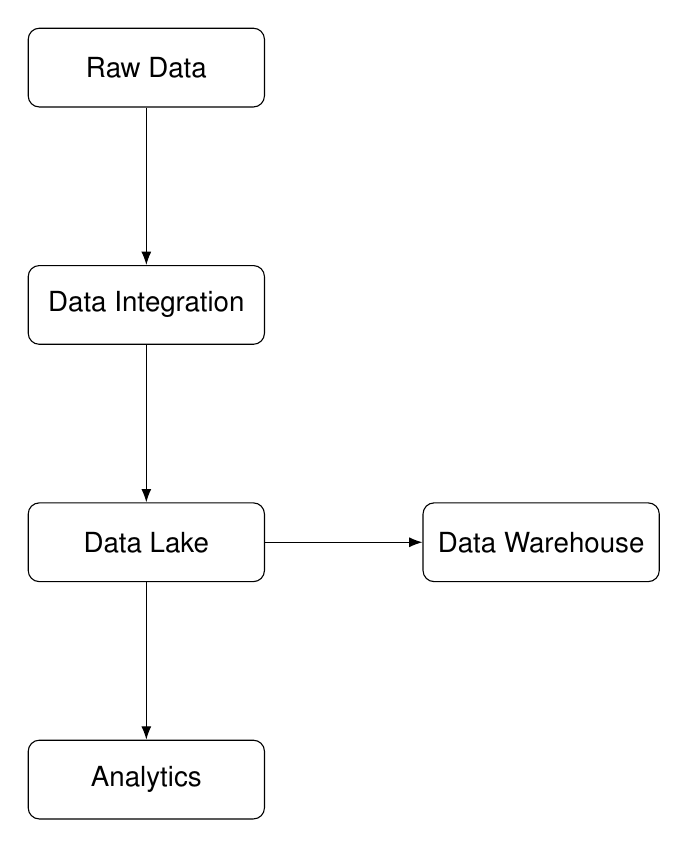
\begin{tikzpicture}[
        node distance=2cm,
        box/.style={rectangle, draw, rounded corners, minimum width=3cm, minimum height=1cm, align=center},
        arrow/.style={-Latex}
    ]

        \node[box] (data) {Raw Data};
        \node[box, below=of data] (integration) {Data Integration};
        \node[box, below=of integration] (lake) {Data Lake};
        \node[box, right=of lake] (warehouse) {Data Warehouse};
        \node[box, below=of lake] (analytics) {Analytics};

        \draw[arrow] (data) -- (integration);
        \draw[arrow] (integration) -- (lake);
        \draw[arrow] (lake) -- (warehouse);
        \draw[arrow] (lake) -- (analytics);

    \end{tikzpicture}
    \caption{Simplified Data Flow Diagram}
    \label{fig:dataflow}
\end{figure}




    \section{Data Types}
    \input{chapters/data_types}

    \section{Data Warehouse}
    %    TODO add additional notes from video

\subsection{Introduction to Data Warehousing}

\begin{note}
    A data warehouse is the single source of truth for the entire organisation.
\end{note}

A data warehouse is generally used to store information from structured data sources.
An organisation collects data from its operational databases and organises it inside a data warehouse, in a format you can perform analytics on.
An operational database is one that holds transactions or data that is written by applications.

\paragraph{Examples to consider}
Examples to consider.
\begin{itemize}
    \item Could have a web shop which collects its transactions in a sales database.
    \item CRM which stores all information in a customer database.
\end{itemize}

Could perform analytics directly on these operational databases.
However, this will impact the performance of your applications.
It will be detrimental to your business if you web shop is running slow, just because some data scientist was querying the data to explore the available features.
It's also the case that operational databases are designed to store transactions and are not easy to query for analytical purposes. (Pretty key point)
Operational databases are designed to be written to, whereas analytical databases need to provide more read performance.
Analytical databases perform better when the data is stored in a columnar format, whereas operational databases are designed for storing transactions in rows.

\begin{note}
    Very key point.
    Makes a lot of sense for any organisation to extract data from all its operational databases and store it in a data warehouse,
    and store it in a way that makes it easy for querying by analysts and data scientists alike.
\end{note}

Companies also enrich their data warehouse with data from external sources.
An example could be combining real time data from the internet with operational data.

\subsection{Datawarehousing for data scientists}

A data warehouse should have an almost perfect view of the entire organisations structured data estate.
It can be a good place to find data to train you machine learning models.
\begin{note}
    If you are struggling to improve the accuracy of your model due to lack of features, it is worth looking into the data warehouse to find additional data.
    Generally speaking users only get read access to the data warehouse.
\end{note}
Also, it is common to impose restrictions on the visibility of data, don't expect all access from day one.

\paragraph{Data Catalog}
Most organisations implement a \textit{data catalog} to provide you with a preview of the data products available in your organisation.
A modern enterprise will not let the data scientists query the data directly but instead ask them to query the data directly, but instead ask them to explore the data sets via the data catalog.
The reality is that most enterprises are not there yet so, data warehouse skills could be in demand.

Once the data scientist finds the data needed for training models, he or she will request data engineering team to transfer it to a data mart or even to a feature store.
This could be a one time transfer ot a transfer set on a schedule.

\paragraph{Example}
A data scientist might request the data engineer to schedule the transfer every week so that fresh data is available on a weekly basis for model training.
The data scientists then use a data science platform or his/her own development environment to engineer new features or pre-process the data for the purposes of model training.

From a data architecture perspective, its important to note that all these tasks are carried out inside the \textit{data mart} or a \textit{feature store} as opposed to inside a \textit{data warehouse}.
Once a model is trained, the inference or predictions are also carried out against the \textit{data mart} or a feature store and not the data warehouse directly.

Data is extracted on a set schedule, which is then sent to the model for predictions.
The predictions are also stored in a data mart which then serves dashboards or applications that utilise the predictive capabilities.
Over of what data warehousing typically means and also how data scientists would typically interact with it.?????

\subsection{Cloud datawarehousing}

\subsubsection{Old way. Data centres. Hardware bundled with proprietary software.}
Old way. Data centres. Hardware bundled with proprietary software.
Data centres were previously filled with these expensive stacks.
On premise data warehouses did perform very well, and they did help organisations derive massive value.
However companies need to make heavy upfront investments to buy, install configure and to maintain these systems and to maintain these systems.
There is also no flexibility either.
They would have to size the data warehouse for your heavy \quote{month end} or quarterly reporting jobs.
This meant that hardware was unused for the rest of the time.

\subsubsection{Cloud data warehousing}
Can trace back the origin of cloud data warehousing.
Cloud data warehouses are hosted natively on public cloud infrastructure as opposed to hardware hosted on premise.
By this it is meant that compute memory and storage managed by the cloud providers.
Moreover, they are usually fully managed and hence you don't need staff to manage this infrastructure or perform software updates for that matter.
All this is managed for you as a bundled service.
This means you can focus on the more important takes, such as loading the data warehouse and extracting the data out of it.

\subsubsection{What differentiates cloud data warehousing from traditional data warehousing}
What differentiates cloud data warehousing from traditional data warehousing is:
Number one, the decoupling of compute and storage, which makes it flexible to have different sizes of data warehouses for different needs and that too is on demand.
Is you have to run a monthly reporting on your data, you can spin up a large data warehouse.
Once that report is done, you can terminate the instance or scale it down to a smaller instance for your day-to-day needs.

\subsubsection{Example: Snowflake}
Snowflake is a popular cloud data warehousing technology.
Uses t-shirt sizing for its sizing in order to make it easier for users to choose the appropriate size for the appropriate time.
Modern cloud data warehousing also supports semi-structured data natively.
Software vendors are trying to support more and more data types making it easy for customers to have just one technology for all data types.
Technology like Snowflake, also strives to cater to multiple use cases.
Instead of using a separate technology for configuring a data mart, feature store and a data warehouse.
The flexibility Snowflake provides allows you to use it for all three purposes.

While specialised feature stores do have an edge, snowflake offers to integrate with them and thus offers the best of both worlds.

    \section{Data Lake}
    
%    TODO add additional notes from video

\subsection{Introduction to a data lake}
A data lake serves as a central repository for all data types, structured semi-structured and unstructured.
They can store ANY type of file in this file system.
The difference though is that the data lake usually offers unlimited scalability, whereas single disk drives are limited.
A data lake is best suited for unstructured and semi-structured data.
There is nothing preventing you from storing structured data in a data lake.
When storing structured data in a data lake, you might wish to consider the pros and cons in comparison to storing it in a data warehouse.
The data lake is a concept.
(Authors opinion) There are three underlying principles that need to be fulfilled by any technology or architecture that calls itself a data lake.

\paragraph{First Principle}
The first principle is that the data lake should support \textit{schema on the read}.
This means that data is not checked for a certain structure or consistency during the write process.
The responsibility or the onus of verifying the data in its structure lies exclusively on the reader.
What this effectively does is that it lowers the difficultly in writing data to almost zero.
As a result you are encouraging applications and users to write any data to the data lake. %Data context
Now this does not have a downside.
You data lake might start off as a clean and pristine storage for data and after a while it might end up being messy.
See data governance

\begin{note}
    To collect data you need to lower the barrier by avoiding schemas on the write and rather applying the schema on the read.
    I.e - Write any data to the data lake, check format when reading it.
\end{note}

\paragraph{Second Principle}
Next principle.
In place analytics
Instead of moving data from one database table to another, schema read makes it possible to read the same data file in different ways.
In place analytics avoids the need for making several copies of the same data set and thus saves storage costs and also the time taken to make copies of the same files.

\paragraph{Third Principle?}
ETL vs ELT
\begin{itemize}
    \item When writing data to a data lake in a data pipeline, data is first extracted and loaded into the data lake.
    \item The loading takes place first and its only then that its transformed based, on the requirements by different users for different use cases.
    \item In comparison, data is extracted and transformed before its loaded into a data warehouse.
    \item When you attempt to load the data, we say that a data warehouse enforces schema on write, while we say that a data lake enforces schema on read.
    \item This is because the data warehouse is generally enforcing a certain structure or schema.
\end{itemize}


\begin{note}
    Authors opinion. These three principles are the most essential principles that must be fulfilled for a technology offering to be classed as a data lake.
\end{note}

\subsection{The technology used to build a data lake}
The most commonly used technology for implementing a data lake is cloud storage.
Cloud storage is offered by all cloud vendors and is sole under different brands.

\subsubsection{Common aspects}
Between some technologies, some aspects are common.

\begin{itemize}
    \item All these technologies offer unlimited scalability on demand so you have store terabytes or even petabytes of data without having to buy install or configure any hardware.
    \item You can/could keep loading data and the cloud storage is expected to keep accommodating it.
    \item Usually you would have to pay for what you store and thus if you apply retention policies on data you can have a good grip on the costs associated with storing data for analytics.
    \item These technologies also offer security mechanisms to protect data and prevent unauthorised access to it.
\end{itemize}

\paragraph{Problems with cloud storage}
Problem with cloud storage is that its only available on public cloud:
\begin{itemize}
    \item Makes it challenging for customers who have data which requires a higher level of protection due to regulatory requirements.
    \item For such customers the Hadoop distributed files system has been a popular choice for a long time.
    \item Hadoop is a distributed computing framework which first appeared around 2006.
\end{itemize}

\paragraph{Hadoop}
Hadoop is an open source software ecosystem that allows you to put together a bunch of computers and build a highly reliable distributed system on top of these computers.
You do not need proprietary software nor expensive hardware, and you can easily create a storage repository which could store petabytes of data at a relatively cheap price.
This would be your own data centre.
The problem with hadoop was that inorder to increase the storage capacity you would need to add more computers or servers to the cluster.
This meant that you would inevitably need to add more CPU and memory which is much more expensive that disks making is hard to scale storage without scaling the other two or vice versa.
This is where object storage offerings form popular hardware vendors start to be more appealing.
\begin{note}
    Important note: In order to avoid vendor lock in you can build your own object storage using software like Minio or Ceph.
\end{note}

These vendors provide proprietary hardware and software technology which bundle much denser and faster disks and are scalable independent of the computer power.
Not only that the object storage vendors usually provide the same protocol of access as the storage vendors.
In effect if you need cloud storage on premise then buying object storage technology is a good choice.

\subsubsection{Summary}
These are the technologies that are commonly used to implement a data lake.

\subsection{Cloud Storage terminology - Buckets and blobs}

The data lake is primarily used to load semi-structured and unstructured data.
There is nothing stopping you from loading structured data as well.
All public cloud providers offer some sort of cloud storage as a service.
See AWS, AZURE etc. Data engineering team will provide a reccomendation for the one you wish to work with.

\subsubsection{Cloud storage terminology}
Cloud storage terminology.

\paragraph{Buckets and blobs}
A bucket which is also referred to as a container somtimes as the name suggests rae logical containers used to organised data.

\begin{note}
    Key point is that buckets cannot be nested.
\end{note}

You can have blobs inside a bucket, but you cannot have one bucket inside another.
Bucket names have to be unique globally.
In amazon, not only does it have to be unique in your account but is also has to be unique globally across amazon.
Data engineers typically create a unique random identifier which is added to this logical name for a bucket.
Also, good to know that buckets cannot be renamed.
So if you were to create a bucket and then wish to rename it you would need to create a new bucket and move the contents form the old bucket there.

\begin{note}
    This could prove to be a hassle if you have stored large quantities of data in the bucket.
    Key point: Best thing to do is to write you code to be agnostic to bucket names.
\end{note}

Another important term is a \textit{blob} which also sometimes known as an object.
All the contents inside a bucket are called blobs or objects and these are immutable.
If you were to try and overwrite an object, a new object get created and the old one gets deleted automatically.

You might see objects that look like directories, these are usually called prefixes.
Behind the scenes, a prefix is also an object.
It has some special attributes which make it look like a directory.
%    Add useful diagram here --- how data scientists would incorporate cloud storage into their data science workflows.
\begin{figure}[ht]
    \centering
    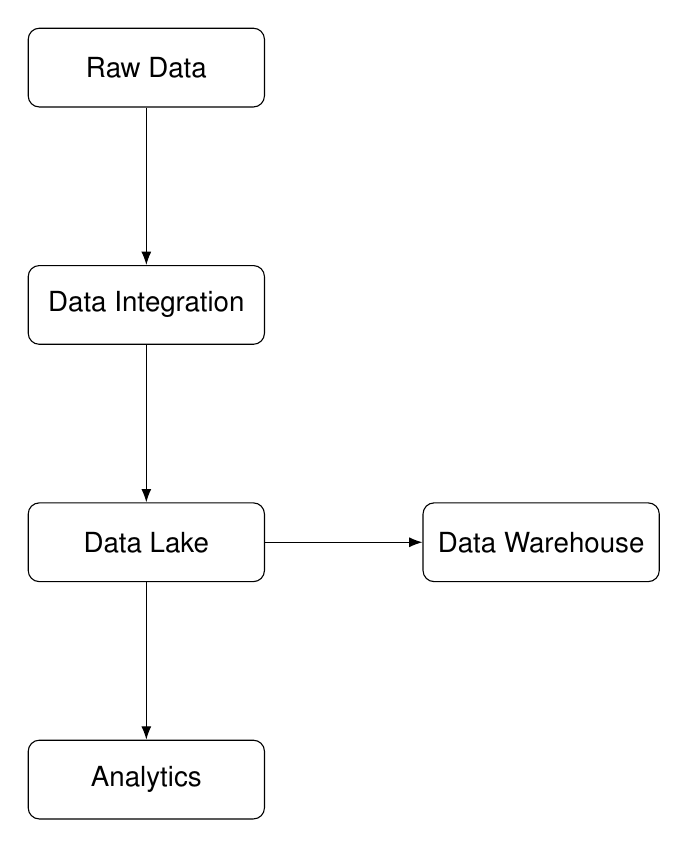
\begin{tikzpicture}[
        node distance=2cm,
        box/.style={rectangle, draw, rounded corners, minimum width=3cm, minimum height=1cm, align=center},
        arrow/.style={-Latex}
    ]

        \node[box] (data) {Raw Data};
        \node[box, below=of data] (integration) {Data Integration};
        \node[box, below=of integration] (lake) {Data Lake};
        \node[box, right=of lake] (warehouse) {Data Warehouse};
        \node[box, below=of lake] (analytics) {Analytics};

        \draw[arrow] (data) -- (integration);
        \draw[arrow] (integration) -- (lake);
        \draw[arrow] (lake) -- (warehouse);
        \draw[arrow] (lake) -- (analytics);

    \end{tikzpicture}
    \caption{How data scientists would incorporate cloud storage into their data science workflows}
    \label{fig:cloud storage}
\end{figure}

One use-case: Can read data directly from cloud storage into your data science platform for training models.
Another use case: Could also use cloud storage for storing data that is used for making predictions, and you could even output the predictions into a file that will be stored in the data lake.
This data lake could be on cloud storage.



    \section{Data Lakehouse}
    
%    TODO add additional notes from video

\subsection{Challenges with the data lake}

As enterprises start finding more and more use cases to derive value from data, they start to explore the possibility of analysing all these data types with the same set of technologies and tools.

\subsubsection{Problems being solved / Need to be solved}
The problem being solved here is the creation of data silos.
Data analysts are generally running their SQL (rigid structure data) queries on structured data and the data scientists are performing analytics using R or python code in the data lake.
The data analysts are hence missing out on the enormous potential of deriving value from the unstructured data and semi-structured data.
The data scientists struggle to lay their hands on valuable historical information in the structured data sets.
One way to solve this problem is to also load the structured data into the data lake.

\begin{note}
    This is technically possible
\end{note}

\subsubsection{What happens if structured data is also loaded into a data lake?}
The first challenge we encounter is that the files we store in a data lake are immutable
This means you \textit{cannot} modify them in place.
You cannot add rows to the same file or modify the roes inside a file without creating a totally new file.
If you're just processing data in batches, this is not a problem.
You can read the file into a computers memory, modify it and then write it back as a new file with new contents easily.

An organisation does not have just batch processing.
\begin{note}
    There is also the need to store and process data that is continuously streaming in, and data lakes are not natively designed to support streaming data transactions.
\end{note}
ACID- Atomic, Consistent, isolation and durability.
Atomicity means that transactions should either succeed or fail completely, or partial transactions can leave data corrupted and unusable.
Consistency means that a file or a data set might be simultaneously updated by multiple applications.
We need some way of guaranteeing the current state of the file.
Isolation is again a simultaneous operation.
They shouldn't conflict with each other, that is what isolation implies.

\begin{note}
    Important: A data lake does not provide ACID guarantees on data transactions made on it.
\end{note}

Finally: Data analysts who are equal stakeholders in deriving value from datasets are traditionally used to querying data using the SQL language and data.
Data lakes do not have native capability to allow such queries.
How to onboard data analysts to use the data lake and store their data?
Build a \textit{data lake house} on top of a data lake

\subsection{Intoduction to the data lakehouse}

Coined by the founders of Databricks. The same company that also created Apache Spark.

\begin{note}
    The term data lake house refers to the combination of two architectures, data warehouses and data lakes.
\end{note}
By combining these two architectures we are enabling users to store and process large amounts of data with increased reliability, scalability and performance.
This concept is constantly evolving.

In its simplest form you need to have three components.
\begin{itemize}
    \item You need to have a Delta Lake
    \item A SQL query engine
    \item A data catalog.
\end{itemize}

\paragraph{The delta lake}
The delta lake is an open source software that helps maintain a transaction log for all the writes being made on files stored in a data lake.
When you write to a file in a data lake that is being access via the delta lake, what happens is that this write is first logged into a transaction log.
Instead of writing directly to the data file, you make a write first to the transaction log and once the transaction is logged to this file the delta lake updates the data file based on a group of transactions that it is has collected.
This way if multiple applications are making changes to the same data set, the Delta lake can decide the order in which the transaction are performed on the underlying files.

This approach provides a number of benefits.
\begin{itemize}
    \item By writing to the transaction log first the Delta Lake ensures that all changes to the table are safely recorded, even in the event of system failures and errors.
    \item Also aids in data consistency.
    \item The transaction log ensures that all changes to the table are written in a consistent order which helps to avoid conflicts and maintain the integrity of the table.
    \item Last but not least we get transaction atomicity.
    \item By writing the transactions to the log before the data fil, Delta Lake ensures that each transaction is treated as an atomic unit of work, meaning that either all the changes in the transaction are written or none of them.
\end{itemize}

Overall, the write ahead logging approach used by Delta lake helps ensure the reliability and consistency of data in a large scala data lake environment.
The delta lake essentially aids in making the transactions carried out on a data lake become ACID compliant.

\subsubsection{Delta Lake features}
\begin{itemize}
    \item Since the transaction lof aids in versioning, the Delta Lake makes it possible to time travel and rollback data to a certain point in time in the past.
    \item It also has a feature which provides the ability to make tables.
    \item You could even enforce the schema or the structure of data that you require applications to adhere to.
    \item This is in contrast to the principles of a data lake which is to have schema on read.
\end{itemize}

\begin{note}
    The delta lake is also designed to query structured data and hence enforcing the schema is sometimes very beneficial.
\end{note}

Along with the Delta Lake which we have already seen you need to add a SQL query engine to the stack,
This can help you data analysts query the tables created in the Data Lake with a language like SQL and that should help in convincing them to use the data lake instead of the data warehouse to store and process structured data.

\subsubsection{Adding a Data catalog}
Finally, to make sure you have good visibility of the data that is landing inside the data lake, It's important to also include a data catalog to this solution.
\begin{itemize}
    \item now this makes it a complete data lakehouse.
    \item You have the Delta Lake maintaining the log of all transactions.
    \item You have a SQL query engine which will facilitate your data analysts.
    \item You also have a data catalog so that everyone has visibility.
    \item Visibility to the data that is stored in the data lake.
    \item Another Benefit \begin{itemize}
                              \item You can perform, merge, update and delete on the data files stored in the data lake.
                              \item You can even use the data lakehouse to directly store streaming data.
                              \item Not with the data lakehouse, you can store your batch data, your streaming data and this could possibly end all the data silos and collaborate better across the entire organisation.
    \end{itemize}
\end{itemize}



    \section{Data Governance with the Data Mesh}
    %    TODO add additional notes

\subsection{Intoduction to Data Mesh}
Establishing the right amount of data governance can be tricky.
If you enforce no governance, your entire data lake or data warehouse will turn into a big mess and discovering useful data sets might become impossible.

\begin{note}
    There are also regulatory concerns, which obliges you do delete someone's data if you are requested to do so.
    Without data governance you organisation could end up paying millions in fines and face prosecution.
\end{note}
The other extreme is having everyone and every project get approvals from a central data team prior to providing access to data.
It also involves constant audits with a burden on the business orientated technology teams to provides evidence of their controls.
While this keeps your data team in control of every decision being made with respect to data governance; it makes innovation impossible.
Primarily due to the delays in accessing data and the data infrastructure and not just for new project but for existing projects.

The idea of a \textit{data mesh} is therefore to strike a balance between the amount of control and the pace required to keep up with innovation and business requirements in side an organisation.

Data mesh is an evolving concept.
At its core.
The goal of domain ownership is to reduce the hops between the data producers and the data consumers, by decentralising certain aspects of data governance.
It's important to start promoting \textit{data as a product thinking} across you entire organisation.

\subsubsection{Data as a product thinking}
\begin{itemize}
    \item A data product is a data set that is discoverable, trustworthy and most importantly valuable on its own.
    \item If all technology decisions need to go through a lengthy approval process, this would make building data products incredibly slow.
    \item It's important to create a self serve platform which has pre-approved architecture and is provisioned automatically.
\end{itemize}

\subsubsection{Decentralised data governance policies.}
Make sure that noone is awaiting the data team's approvals for accessing data or even publishing data products in the data catalog.
Data should be checked automatically based on predefined policies and compliance checks need to be done with the help of automation.
Technology is available to implement such automation such that it facilitates establishing all the four principles that have been described without the need for human intervention.
What is actually needed is the organisation will change the culture to make it happen.????

\subsection{Data mesh principles: Domain ownership and data as a product}
If you do not have a data mesh implemented in an organisation then the situation might resemble the illustration (add diagram)
All the responsibility of extracting, processing and governing the data therefore lies solely in the hands of the central data team.
All the stakeholders who would benefit from having access to data need to consult the central data team.

\begin{note}
    Be aware of how long it take for access to the data in such an organisational structure.
\end{note}

\subsubsection{Data mesh}
The data mesh on the other hand relies on the principle of \textit{domain ownership} of the data.
You have the \textit{source domain}, which is the organisation that produces the data.
This could be a product team that has created some microservices.

Essentially, these are the people running the operating systems and maintaining the operational databases.
Followed by the source domain is the \textit{consumer domain}.
This is the organisation that consumes the data for analytical purposes.

\subsubsection{Example}
Data is produced by the web shop is consumed by the marketing analytics team, would in turn created data products that will be consumed by the data consuming applications.
By that it is meant dashboards and business KPIs.
The ownership of maintaining the source data lies with the source domain and the ownership of the analytics data.
Product lies with the consumer domain.
The reason for not combining the two domains is that the folks in the source domain area already burdened with work relating to keeping the applications running 24-7.
It's also a fact that these people are no experts in analytics.
In essence we are getting rid of the need for a central data team to make decisions and act on them.
If the source domain makes changes to their application and starts producing data in a different format, the consumer domain can directly communicate with them and decide on the course of action.
Empowering this entire structure is the \textit{domain agnostic data platform}, which offers self-service tools to all the domain and data consuming applications.
There ism thus still a need to have a central team whose responsibility now is to create automation and standard practices that empower the domain teams.
By doing so the central team now acts as a facilitator and not as an inhibitor.

\subsubsection{Promoting data as product thinking}
Promoting data as product thinking
To understand this, we need to outline the role of a data product owner.
A data product owner has end to end ownership of maintaining the value of the data product.

Product owners therefore need to be incentives to maintain and also augment the value of the product they are responsible for.
They are also responsible for improving the discoverability or their assets.
Future trend. Data product owners. (Author opinion)

\subsection{Data mesh principles: Self service and federated governance}
There is a some amount of centralisation, even in a decentralised approach like a data method.
The data platform team now has the responsibility of creating self-service tools as part of the domain agnostic data platform.
These tools will help domain teams create and maintain their data products independently.
The data platform team creates a self provisioning unit of the platform, which has the essential storage and computer technologies needed for storing and processing the data.
There also come with automated polices which will ensure that the infrastructure is used as per the security guidelines of the organisations.

\subsubsection{Example}
The self provisioning unit will contain a policy which prevents you form making the contents of your cloud storage bucket public.
What this essentially means is that it will inhibit the domain teams from accidentally or intentionally making the data visible on the internet, and thus preventing it from landing in the hands of hackers and other malicious elements.

\subsubsection{Federated computational governance}
What is essentially means is that the data mesh does not rely on manual checks and audits to enforce governance because if you had manual checks and audits it would again slow down the innovation that relies on data.
Instead, the data mesh relies on technology to detect and enforce the relevant policies and prevent the misuse of data.
It also makes sure that the data products have the necessary metadata so that they are easily discoverable.

\paragraph{Examples}
Your data platform team might create a policy which check for personal data prior to authorising permission for use of this data in machine learning projects.
Using personal data in machine learning projects makes them subject to additional compliance requirements and hence it's best to use features that don't contain personal information to train machine learning models.

Another example would be to enforce mandatory information to the metadata of a dataset.
\begin{itemize}
    \item This helps you to better discover the dataset when it's published in the data catalog.
    \item This helps you to better discover the dataset when it's published in the data catalog.
    \item This information should help you decide if an organisation is in need of a data mesh or not.
\end{itemize}

\subsection{Data Catalog}
The data catalog is ideally the only place you need to visit to find, understand and govern data.

\subsubsection{How would you know if some data exists?}
In the traditional approach, you would ask your colleagues or search for some documentation on your intranet to seek such information.
Could give your employees full access to their data infrastructure for them to find such information.
This can be quite risky approach from the perspective of data governance.
A better approach is to establish a data catalog.
Publish your data in a catalog.

\subsubsection{The top three features a data catalog is expected to fulfil are}
\begin{itemize}
    \item Data search and discovery.\ It should aid users to simply search for information and find data products that might contain the data they need. Once the user finds the data product, the data catalog usually provides a preview of the data set with some sample data that helps the user understand if this is useful for their next project.
    \item Next up, data catalogs can display the metadata of the data set, for example the freshness, the frequency of updates and sometimes the metrics on data quality. This means you can ensure that your project is accessing the best and the most trusted data source that your organisation has access to.
    \item You could also enforce data governance via the data catalog. The data catalog could detect if the data set has personal data and tag it as not fit for machine learning projects.
\end{itemize}

Ultimately, the data catalog facilitates collaboration.
The best data catalog software out there provides the capability of adding wiki like pages to your data products.
You could also leave comments next to the product page to build tribal knowledge about the data set, which might prove useful to the entire company and not just your team.
See google big query.

\begin{note}
    Data catalogs are a big topic.
\end{note}

\subsection{Data Contract}
Revisit the principles of a data mesh within a data mesh frameworks.
The source domain, or the creator of the data provides data to the consumer domain.
The relationship necessitates that the consumer domain relies on the source domain to maintain the data schema or format.
Consequently, the consumer domain in turn serves as a source for applications that consume data from the domain, establishing a provider-consumer relationship between entities within an organisation.
Now, this structure facilitates the creation of data products that are both independent and autonomous.
However, it also introduces the risk of changes that occur in one domain adversely affecting another.

\subsubsection{Example}
If the source domain decides to delete a column from the data set it was maintaining, applications or data pipelines in the consumer domain will fail due to their reliance on that columns' presence.
To mitigate such risks while preserving autonomy, the concept of a \textit{data contract} has been introduced.
Data contracts act as intermediaries between domains to ensure that no breaking changes are made by one domain that could negatively impact another.
Data contracts are a set of rules designed to maintain harmony between the domains.
Verbal contracts involve agreements on data creation and maintenance to prevent pipeline disruptions.
However, the reliability of verbal agreement is questionable in today's context.
Written contracts offer a more tangible solution by documenting the agreed upon schema and data types.
Written contracts are simply some data documents that are written rules that are maintained on a wiki page or confluence.
Though without enforcement, the risk of non-compliance remains.

Automated contracts therefore emerge as the optimal solution.
They act as checks and balances, verifying alignment with agreed upon formats as data is created, written, read and thus preventing unplanned outages and ensuring integrity of data products.

\subsubsection{Sample data contract}
Uses YAML like syntax.
INSERT EXAMPLE
Can use regular expressions to enhance the robustness of these verifications.
Goal: to consider is target data cleaning and enhance the quality of the data set.
Scrutiny is very important for the analysis of data that is relies on stability and consistency of relationship over time.
Data contracts can span from a few lines to extensive documents, pointing a future where advancements might enable large language models to autonomously generate data contracts based on data set observations.
Enforcing these automated data contracts is a critical step in the process.
When the source domain contributes data to a data lake or data lake house, it must pass through these automated validations to ensure compliance with the desired formate.
Similarly, when the target domain retrieves data, it undergoes a verification process via the data contracts; guaranteeing that the extraction aligns with pre-established agreements.

Used data contacts to enforce quality of data (check)

\subsection{Data Fabric}
Architectural framework that has emerged from the data mesh. \textbf{Data fabric}.
Helps implement the ideals of the data mesh.
When implementing a data mesh in an organisation, the goal is to democratize data and analytics, which allows for the extraction of value from data.
This approach lets business units choose the tech stack they are most comfortable with.
Ideally there should be a standardized tech stack within the organisation, but in reality organisations often have diverse tech stacks.

\subsubsection{Tech stack diversity challenges}
This diversity leads to various challenges.

\begin{itemize}
    \item First challenge is data silos. Each team may have its own infrastructure creating data silos. Works fine in a department, but hinders collaboration and creation of cross departmental data products.
    \item The second challenge is data duplication. Creating data products from different departments often requires copying data into new infrastructure leading to multiple data copies. This duplication increases costs and governance overhead. Different departments might store data in various formats, requiring extra efforts to unify these formats for analysis.
    \item User experience is another challenge. Diverse technologies mean users must learn new tools and languages to access different data sets. This slows down analysis and reduced efficiency. Additionally, each department has its own authentication framework and this complicates access control for integrated data products.
    \item Security and governance is also a challenge. Different technologies have a unique security and governance implementation and unifying these controls across an organisation can be extremely challenging.
    \item Monitoring and managing audit logs can be complicated due to the requirement to gather them from diverse technologies.
    \item Billing and licensing across a diverse data landscape can make it hard to visualise the costs and keep control on it.
\end{itemize}

To address these challenges, technology providers have developed the concept of a \textit{data fabric}.
This framework overlays existing environments, whether they are on premise, cloud or hybrid without requiring data migration.
It aims to make the governance more sustainable.

In the Data Fabric architecture, data can be hosted in various environments such as data lakes, data warehouse, databases and big data infrastructure.
The first step is the automated collection of metadata from all the data sources.
Building a semantic layer on top of this metadata is crucial.
This layer creates business specific data models, allowing for, e.g.\ sales and marketing teams to create different data models using the same data set.
A knowledge graph connects data across data sets, creating a graph of entities and their relationships.
Data catalog and profiling tools help managed and organisation the data.
The semantic inference layer, powered by AI and ML allows users to query the data using natural language, making it easy to interact with the data.
Data virtualization unifies access to data across, different technologies enabling users to run queries without learning new languages.
The semantic query layer simplifies data queries with interfaces similar to ChatGPT\@.

These are the benefits of the data fabric and they are very significant.

It enables effective data governance processes and reduces the effort needed for data integration, since data is not moved between silos.
Now business users can easily discover and access data; improving business processes while data scientists can use data across silos to create recommendations and machine learning applications.

Overall the data fabric framework enhances the ability ot manage and utilise data across the organisation.

\subsubsection{Summary}
The data fabric addresses the challenges of implementing a data mesh by providing a unified layer for data governance, access and integration.
This ensures that data remains accessible and useful across the organisation regardless of the underlying technology stack.

Azure Fabric.
Admin users can access a view of all data assets.
One data lake can abstract everything and provide you with a universal way of accessing that data.

You have monitoring.
Here you can see the audit logs which are gathered from all the users actions that happen on the platform.
You have the real time hub where you can actually integrate real time data streams into your databases or into your data lakes.
You have workspaces that allow you to collaborate on your data sets with other departments etc.

Semantic data models.
Basically create a business view form a business perspective. The view can be shared with others.

There also generative AI components. Can be used to create the charts automatically.

TODO - checkout microsoft fabric



    \section{Streaming Data in Data Science}
    
\subsection{Introduction to streaming data}

Streaming data refers to the continuous real time flow of data from various sources.
This produces data at a high velocity.
Unlike batch data processing, streaming data \textit{has to be processed in real time}.
Batch processing is done periodically.
Could schedule a batch job to run every night or daily once or run every few hours and at best run every hour.

\begin{note}
    The expectation with real time data is that the data gets processed every few seconds or at least every few minutes.
\end{note}

Hence, the two techniques.
They need different approaches.
Typical uses cases where real time processing of streaming data play a big role are payment fraud and the finance domain.\ Particularly banks.
AML is closely relate to payment fraud but only requires batch processing.

Predictive maintenance use cases which involve anomaly detection is one of the common data science use cases which is found in the manufacturing industry.
Data from senors has to be processed in real time and predictions made on the likelihood of failure of the equipment.
Manufacturing and industrial IoT have a lot of other use cases as well where one has to deal with streaming data.

\subsection{Kafka 101}

Most streaming data use cases employ kafka in some form or the other.
OS software for implementing a distributed platform for supporting high throughput streaming data.

\subsubsection{Kafka - Terms}
\begin{itemize}
    \item Producers: Data sources which generate the streaming data. Configured to write data into several topics
    \item Brokers: Topics are distributed on multiple kafka servers which are known as brokers. A kafka cluster will have at least three brokers to ensure fault tolerance and to prevent the loss of data in case of failure of the servers.
    \item Consumers: Applications that read data from the topics which are hosted on the brokers are called consumers. Training models can be making predictions or what is called doing inference.
\end{itemize}

\subsection{Lambda architecture}
The most commonly deployed architecture in the industry for real time or streaming data use cases is the lambda architecture.

In this setup the streaming data is first ingested into distributed streaming platform such as Kafka.
Data from different sources is stored in several topics hosted on the kafka brokers, inside a kafka cluster.
Simultaneously we set up a data processing job that runs continuously, reading and processing data from the Kafka topics.
The most commonly used frameworks for processing streaming data are Spark and Flink.
The data processing job Utilising these frameworks will output the processed data into a data lake house and, simultaneously send this data to a deployed model for making predictions.

\begin{note}
    The properties of a data lake house make it suitable for streaming data.
\end{note}

The data in the data Lake house is then used for training the models.
What this effectively means is that hte training does not happen directly by reading the data from kafka.
Rather by utilising the data stored in a data lake house.
Now, once the model is trained it can be deployed on to a model serving platform.
The deployed model then makes predictions in real time on the data that is sent by the data processing application.
The predictions can then be used by downstream applications.

\subsubsection{Examples}
Could be dashboard that displays anomalies, or it could be that we store the predictions in a database for use in the future.

\subsection{Kapppa architecture and comparison}
Lambda architecture has several limitations.
Kappa architecture was evolved to solve these problems.
General opinion is that Kappa architecture should be the default for Batch, Streaming and for all Data Science projects.

Reasons for this is that it caters to both batch and read time uses cases within the same template.
Its also believed that instead of extracting data from data sources in batches, the future entails all data sources to be streaming data in real time.

\subsubsection{The Kappa architecture}
Just like the Lambda architecture relies on data sources sending their data to a streaming platform, like Kafka and similar to the Lambda architecture.
Here too, the data is stored inside Kafka topics and hosted on Kafka Brokers.
The difference is that model training is performed by utilising frameworks like TensorFlow which can plug in directly into Kafka and read data from the topics hosted on it.
Kafka has a very central role in the architecture and it's common to use a technology called kafka.????
Streams also send the data to the model for making predictions.
Now subsequently, the data is offloaded from Kafka and stored in a data lake house for use by applications performing batch data processing.
This data can also be used to uncover trends in the data over a longer period.
This is in contrast to the temporary nature of data analysis in a streaming application, for example that detects anomalies in real time.

\subsubsection{Lambda vs Kappa architecture.}
Lambda architecture is more prevalent and has been around for longer time than the kappa architecture.
Hence the know how for implementing it is more readily available over the Kappa architecture.
Because of its maturity almost all machine learning frameworks support the lambda architecture.
After all, you will be training models with the data that is available in a data lake house or a data lake, which is something all ML frameworks tend to support.

The disadvantage of adopting the Lambda framework is that one has to read and transfer data from the Kafka topics to the Data Lake House in order to train the models.
This can lead to some delays in the making the training data available to the models.
This does not fall in line with the expectations, in some of the cases where customers would like to train models almost in real time.
Such needs are quite rare though and hence the lambda architecture servers quite well for most use cases.
The Kappa architecture has the advantage in that it caters to both batch and real time use cases.
Though it does require that you stream all your data to a streaming data platform like Kafka, making Kafka the central data fabric of your data architecture.

The disadvantage of adopting the Kappa architecture is also that not all frameworks support direct integration with Kafka.
At the time of recording, only TensorFlow has support for such an integration.
Additional support will be added over time.
This means that you have additional overhead in developing and maintaining such applications.
The belief is that we shall see more and more of this architecture being adopted.
Expect to come across lambda architectures more often.

%    \subsection{Word of caution and Resources} --- TODO find my own




    \section{Data infrastrcture for Machine Learning}
    
\subsection{Feature Store}
Several tools have emerged to improve the efficiency of machine learning workflows.

TODO see diagram
Will observe that for each use case, the features have to be extracted and engineered separately.
Not only that, engineered features cannot be reused in multiple use cases.
Instead, its common practice that each data scientist or data scientists within a team perform feature discovery and feature engineering every time they embark on developing a use case.
That can be a colossal waste of time and effort.
This is when it makes sense to implement a \text{feature store}.
A Data scientist could request to the data engineering team to extract the required features form the data warehouse or the data lake and the perform feature engineering inside the feature store.
This speeds up the machine learning life cycle considerably.
First it reduces the dependency on the data engineering team to repeatedly extract a feature for you.
Once you have identified the features, you could request the data engineering team to setup a pipeline to extract and load the features into a feature store on a set schedule.
Once the features are available in the feature store, you as a data scientist could engineer new features independently of the data engineering team.
Having a feature store, also aids in collaboration with other data scientists in your organisation.
The effort you have put into engineering features can be reused by your colleagues and vice versa.
You could find and reuse feature engineered by your peers and save a ton of effort while still improving the accuracy of your model considerably .
Now the feature stores are not just useful in speeding up use-case development or model training but also sometimes or even imperative on the inference side.

When I say the inference side, I mean the phase where you have deployed the model and where it is making predictions.

\subsubsection{Example: Payments fraud detection is a common use case in the banking and finance domain}
Whenever a transaction is made it is sent to the model that is deployed to classify your transaction as either safe or as fraudulent.
To make this classification, it is not enough to just give the model details of the transaction.
If the model were to make the decisions based on just the transaction information, it will very likely classify it as a false positive or false negative.
If you provide the model additional features such as a location, engagement data device mapping etc you could get better classifications.
Without a feature store, the inference pipeline would have to gather and compare all these features form different data sources.
It would be an impossible task.
Rather, what is generally recommended is to gather and compute all the necessary features at least on a daily basis.
Each night data pipelines will extract and engineers the features for each customer record and the store is in the feature store.
Then when the transaction is actually made all that has to be done to combine the information with the ready made features inside the feature store.
Having the feature store is also important because the prediction for such a use-case needs to be made in a few milliseconds.
I.e that is in real time.
Without the features being present in the feature store, it would be nearly impossible to make all these computations in a few seconds or even a few minutes.

\subsection{Vector Databases}
Vector databases are designed to store the embeddings of different types of data like text, audio and images.
You could also create vector embeddings of videos as well.
Not only that, vector databases allow you to perform a \textit{vector similarity} search to find similar vectors.
To understand vector databases, we need to understand what a vector embedding is.
Simply put, a vector is a special way of showing information about something using numbers.
Essentially, they are a set of numbers that capture the meaning and relationships between different items.

The resulting vector embeddings can be used in a variety of natural language processing tasks such as sentiment analysis, machine translation and text classification.
There are other neural networks, each specialised in creating embeddings for different types of data.

Once content is vectorised, you can perform a vector similarity search on a database of vectors.
There are various types of vector search techniques, not just one.\ One example.......cosine similarity.\ Use an angle to measure how similar things are.

\begin{note}
    That most text embeddings will be at least a few hundred dimensions instead of just two.
\end{note}

\subsubsection{Useful Examples}
Can use it for finding similar images based on their vector embeddings.
Same with text.
Can also be done with semantic content in documents.
Can be used in law enforcement etc.


    \section{Flowchart and Use case examples}
    \subsection{Data Architecture decision making flowchart}
See diagram.

\subsubsection{First question - batch or real time}
If data needs to be precessed every day or evey few hours then this is a batch scenario.
Where is if data processing is required every few seconds or minutes we looking at a case of real time data processing of streaming data.

\subsubsection{Next question, what kind of data are we dealing with}
Could be structured, semi-structured unstructured or a mix of all these.
In the case of a mix it can be called multi modal data.
If its a use case that involves only structured data, then you could choose between a data-warehouse or a data lake house to store and process your data.
Theres nothing stopping you from using a data lake but these two will be much more efficient when dealing with structured data.

If you're dealing with semi-structured data or unstructured data then the choice is between a data lake and a data lake house.
Some data warehousing technologies have also adapted very well to processing semi-structured data.
This is an option that is worth exploring

You may come across NoSQL databases hosting semi-structured data but author has rarely come across them as being useful for performing analytics.
They are primarily used to serve data to applications.
If you data is a mix of different data types perhaps you have structured data in database tables and images form user reviewers, or may have a mix of geoJson and text.

In all these scenarios, it will be wise to choose between a data lake house or a data lake.
The data lakehouse obviously offers a lot of benefits over a simple data lake.
On the other end of the spectrum if your use case needs real time data processing then you need to consider the \textit{frequency of model training}.

\subsubsection{Machine Learning considerations}
Does your use case require training and retraining models daily or every few hours?
Does it require training and retraining every few minutes.
Online training of models is still quite a complex process to build and is undertaken quite rarely in the authors experience.

If you model training frequency is not so demanding then you could implement the Lambda architecture for processing streaming data.
If you use case demands online training or training directly on streaming data then the Kappa architecture would serve you well.

There is a push towards unifying batch and real time data processing with the Kappa architecture and this is to avoid creating different tool sets for two different data processing patterns seen so far.

\subsubsection{Data governance considerations}
Worth enquiring about data governance in your organisation.
Does your organisation have a data mesh implemented or is there a data catalog where you could find data products.
How long does it take to get access to the data lake and many other aspects that could queried or inquired right at the onset of the use case development.

\begin{note}
    Making these inquiries at a later stage could delay your model being productionsied.
\end{note}

Worth enquiring about the availability of specific data infrastructure.
Does your IT team have the possibility to provide you a feature store.
Because in some cases it would be imperative to use feature store to realise a use case.

\subsection{Use case examples and applying the decision}


    \chapter{Glossary}

\end{document}